\subsection{Product View}

The \emph{Product View} is based on a common approach used in product management, a \emph{product tree diagram}.
The Documentation Working Group developed a framework customized for Rubin Observatory operations to facilitate the development of documentation and effective communication consistently project-wide.
The two primary purposes are to convey ownership and responsibility of technical documentation and more readily describe complicated systems with context and categorization.
The Product View allows one to identify specific documents as the normative source of information, then provide a manner which one can associate, link and cross reference documentation and informational dependencies from respective normative sources or references thereafter.
These goals support identifying and resolving gaps, miscommunications or error-likely situations.
The expected primary users are managers, product owners, engineers, specialists, technicians, and users who want to search downwards in a system's hierarchy.

The Product View will consist of product trees developed by the owning \emph{Rubin Observatory Departments}, their technical teams and product owners.
Each department's product tree(s) should be constructed to best organize and compartmentalize the set of \emph{products} that make up the suite of complex systems under their purview.
Products can span all manner of objects, such as department-specific categories, documents, hardware (systems, servers, networking, etc.), data (data sets, validation tests, verification artifacts, etc.), software interface information (alarms and notifications between hardware or software systems, support data storage and metadata schema, etc.), or subject-matter expert support.

Each department or group is responsible to manage the product trees in addition to updating technical documentation to support access to retrieve associated information, interfaces and requirements with consistency and reliability.
In light of this need, the Documentation Working Group recommends all Product View trees be available via one of the project repositories --- it is suggested to create an appropriate lsst.io website so departments and groups can easily make changes.

Products are defined by the owning department in terms of a system or set of systems which can be grouped or decomposed into subsystems or individual components that is appropriate for them and their stakeholders.
Referred to as the \emph{generic categories}, the customized categories for the Product View developed by the Documentation Working Group are predefined root-nodes and the first set of leaf-nodes for a product tree.
The generic categories were developed to capture critical operational aspects of a product while being extendable to subsystems of a product, where the subsystem may be a product with subsystems in its own right; i.e., a \emph{Level-1 product} can be comprised of multiple Level-2 or lower-level subsystems, and those subsystems which are products are \emph{Level-2+ products}.
Note that these terms do not correspond to the construction phase definition of Work Breakdown Structure (WBS) or colloquial "subsystem" used across the construction project.
It is at the department's discretion on how to best organize and characterize these products and their product trees to manage their systems and flow of information; however, it is expected that all generic categories are associated with Level-1 and Level-2+ products either by construction or referenced information.
While there will be exceptions for low-level systems, the Product View and its generic categories are designed to robustly capture construction completeness and operations readiness because they should generate sufficient discussion between groups and stakeholders to ensure key information is identified and provided.

\subsubsection{Departments for Rubin Observatory operations}

The Rubin Observatory departments shall be described by their associated scope, systems and/or products descriptions, and contacts to identify managers, product owners, or other key personnel (e.g., organizational chart, contact list).
This section lists each department and respective scope.
Contact information should be available to individuals that require it, and it should be clear when it's appropriate to contact an individual or group (e.g., as a product owner).
Note that sometime \emph{R} prepends these acronym, e.g., ROO for Rubin Observatory Operations.

\textbf{Director's Office} (DO) ---
The Vera C.\ Rubin Observatory Director's Office is responsible for the overall management of the observatory and the LSST survey, as well as fulfilling the mission of the observatory and realizing its vision.
The Director's Office includes a Directorate, Administrative Operations, Safety, Communications, and In-Kind Contributions teams.

\textbf{Observatory Operations} (OO) ---
The Chilean-based Rubin Observatory Operations Department is responsible for operating and maintaining the telescope, camera systems, and summit facilities in order to collect the raw imaging and housekeeping data needed by the LSST.
The primary tasks include maintaining the operating facilities, conducting the night-time survey operations, real-time assessment of image quality and observing efficiency, performing the daily calibration, and collecting and analyzing engineering data.

\textbf{Data Management} (DM) ---
The role of the Rubin Observatory Data Management department is to accept data from the Observatory's telescopes and ancillary systems; to process that data to generate science ready data products; to archive both raw data and derived data products; and, subject to approval from the Science Performance department and the Data Release Board, to make that data available to the scientific community.
The Data Management department will develop, maintain and operate the networks, compute and storage hardware, and software that constitutes the Rubin Observatory Data Management System for the duration of the operational period.

\textbf{System Performance} (SP) ---
Rubin Observatory System Performance department is responsible for ensuring that the LSST as a whole is proceeding with the efficiency and fidelity needed to achieve its science requirements at the end of the 10-year survey.
This includes the Wide-Fast-Deep (WFD) survey and all Special Programs (deep drilling fields and mini-surveys).
To meet this goal, the System Performance department will track and optimize the integrated performance of the entire system.
This includes the performance of the observatory and the progress of the survey with respect to its science objectives, the ability of the community to access and analyze the data and publish results on the four LSST science pillars at an appropriate rate, the evaluation of strategies for improving the survey strategy, and the development of mitigation strategies together with other relevant departments to minimize the impact of changes in the system performance on the overall LSST science.

\textbf{Education and Public Outreach} (EPO or EP) ---
The mission of the Rubin Observatory Education and Public Outreach program is to offer accessible and engaging online experiences that provide non-specialists access to, and context for, Rubin Observatory data so anyone can explore the Universe and be part of the discovery process.
EPO serves as a website that highlights and contextualizes the scientific power of Rubin Observatory for non-specialists and hosts all online resources.

\subsubsection{Generic Categories for the Product View}

The generic categories provide a basis to define and associate critical systems and objective elements of a department and associated systems; they are not products in themselves.
They are designed by the Documentation Working Group to relay information in a complete and concise manner by standardizing the distribution of information and products.
Further opportunities arise with a well designed set of product trees: clearly establish relationships and dependencies between systems, serve to introduce the department/system in a digestible manner, and create a more adaptable structure to organize and target information between technical groups internal or external to the department.

The generic categories are separated by five high-level categories that act as root-nodes --- Technical Design, Procedures, Safety and Emergency Response, Evaluation and Archival Documents.
Each one includes subcategories that are the first- and second-level leaf-nodes.
The generic categories are applicable to a variety of systems (e.g., hardware-centric, software-centric, hardware and software distributed, process and protocol dedicated) such that information associated to these categories and subcategories are available for practically all systems or subsystems described via a Product View tree.
It may be difficult at first for technical groups to perform a logical and relevant decomposition of the systems such that the generic categories are applicable to all product trees, especially if a system can change in different scenarios, contexts, or states (e.g., the Simonyi Survey Telescope could have a product tree for maintenance and a different product tree for on-sky operations where each capture different components and interdepartmental interfaces separately).
However, even in the case where the owner and stakeholders agree a category doesn't apply, the generic categories are a way to define and describe scope, respective responsibilities, inter- and intra-departmental interfaces, requirements, and key expectations.

Teams can and should create product trees that refer to documentation and ensure the product tree describes how these external documents address the generic categories.
For example, this can take the form of a diagram coupled with a narrative, potentially with different representations between leaf-nodes.
Within the Product View as a whole, consisting of many product trees, it is intended systems and subsystems refer to higher- or lower-level product trees to reduce replication and the risk of confusing users accessing information between the group(s) and stakeholder(s).
Furthermore, the referential nature can be applied for interdepartmental information and dependencies so it's clear which department owns the information and any departments which utilize it.
For example, an interface control document (ICD) and an N-squared diagram could be sufficient references to describe the category \textit{Inter-department Interfaces}.

Here are the generic categories:

\begin{small}

\begin{itemize}
  \item Technical Design
	\begin{itemize}

	  \item System Description
		\begin{itemize}
		  \item Description of System(s)
		  \item Definition of Sub-systems
		\end{itemize}

	  \item Technical Design Specifics
		\begin{itemize}
		  \item System-level and Intra-department System Interfaces
		  \item Sub-system Level Information
		  \item Inter-department Interfaces
		\end{itemize}
	  \item Access Interfaces (Physical and/or Software)
	\end{itemize}


  \item Procedures
	\begin{itemize}

	  \item Operational Procedures

	  \item Maintenance Procedures
		\begin{itemize}
		  \item Preventive Maintenance
		  \item Reactive Maintenance
		  \item Turn-over Protocols (e.g., shift change, operational-to-maintenance status change)
		  \item Sub-system Isolation
		\end{itemize}

	  \item Software Access and Use Documentation for Users

	  \item Software Development Documentation for Developers

	  \item Manuals and Data Sheets
	\end{itemize}


  \item Safety and Emergency Response (System-level and relevant Sub-systems)
	\begin{itemize}

	  \item Emergency Procedures and Contacts

	  \item Hazards and Hazard Analysis

	  \item Mitigations and Verification Artifacts
		\begin{itemize}
		  \item Protocols
		  \item Energy Isolation
		\end{itemize}
	\end{itemize}


  \item Evaluation
	\begin{itemize}
	  \item Performance

	  \item Failure Effects and Failure Mode and Effects Analysis (FMEA)

	  \item Validation/Verification Test Plans

	  \item Test Reports
		\begin{itemize}
		  \item Technical Reports (Test and/or Analysis)
		  \item Verification Reports
		\end{itemize}
	\end{itemize}

  \item Archival Documents
	\begin{itemize}
	  \item Communications (e.g., Request for Information [RFI])
	  \item Construction Information, Unrelated to Commissioning/Operations
	\end{itemize}
\end{itemize}

\end{small}

\subsubsection{Examples of Product View trees}

Here are two examples of product tree referencing, using Auxiliary Telescope (AuxTel), LSSTCam and Commissioning Camera (ComCam).
Note that it would be beneficial to design product trees which take advantage of the similarities between LSSTCam and ComCam, even though there will be major differences, too.

For these three systems, the Access Interfaces category would include a common set of software, e.g., LSST Observing Visualization Environment (LOVE), Nublado (Jupyter) interface, Script Queue, Watcher.
This common set of software could be included in a higher-level product tree (potentially a Level-2 product under the Observatory Operations department) or as a referential Level-2+ product trees; then, not only is the information referenced to all three efficiently, but the software product tree(s) can be designed to easily indicate differences between the three systems, say, for the Software Development categories.

The three systems interface with a set of external systems simultaneously connected to them, e.g., Engineering Facility Database (EFD), Environmental Awareness System (EAS), Global Interlock System (GIS).
These external systems could also be set up as referential product trees which are referenced by AuxTel, LSSTCam and ComCam, as well as others.

Figure \ref{fig:product-view-departments-example} depicts the Rubin Observatory departments and a subset of their systems and products into Level-1 products, with some Level-2+ products included.

\begin{figure}[htp!]
\centering
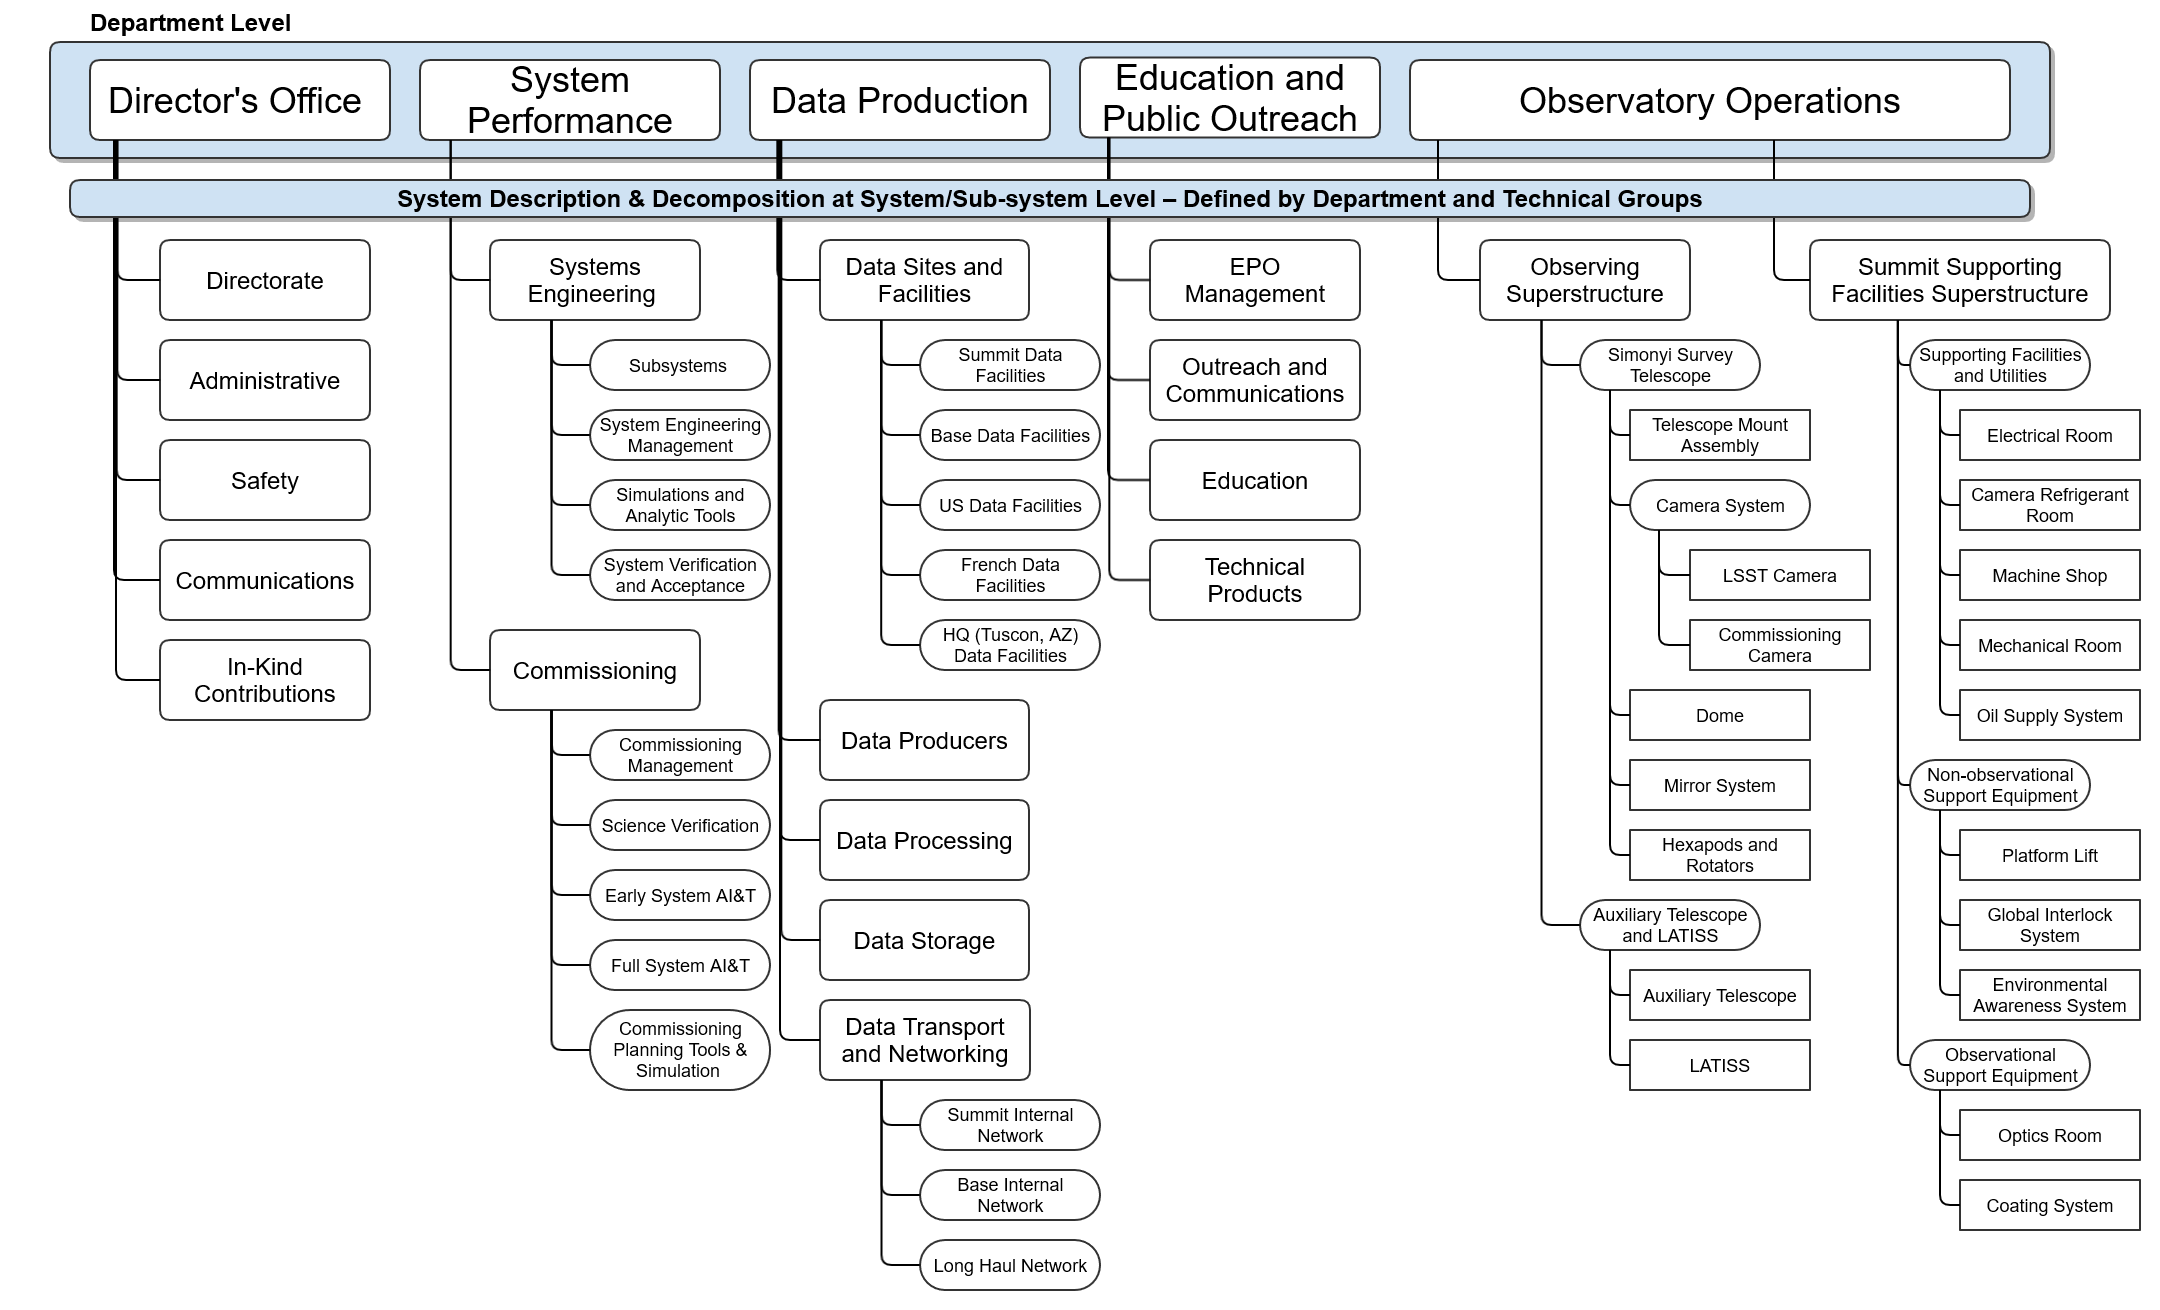
\includegraphics[width=\textwidth]{product-view-departments-decomposition-example}
\caption{Example of Department Decomposition at System and Subsystem Level.}
\label{fig:product-view-departments-example}
\end{figure}

Figure \ref{fig:product-view-auxtel-technical-design-example} is a more comprehensive example of AuxTel, depicting the Technical Design generic category.
Each category (yellow) and each subcategory (blue) from the Technical Design is addressed such that the reader has an idea of what the system is, how it is used, and documentation with references therein for retrieving critical information.
Note that physical interfaces are not address in the example.

\begin{figure}[htp!]
\centering
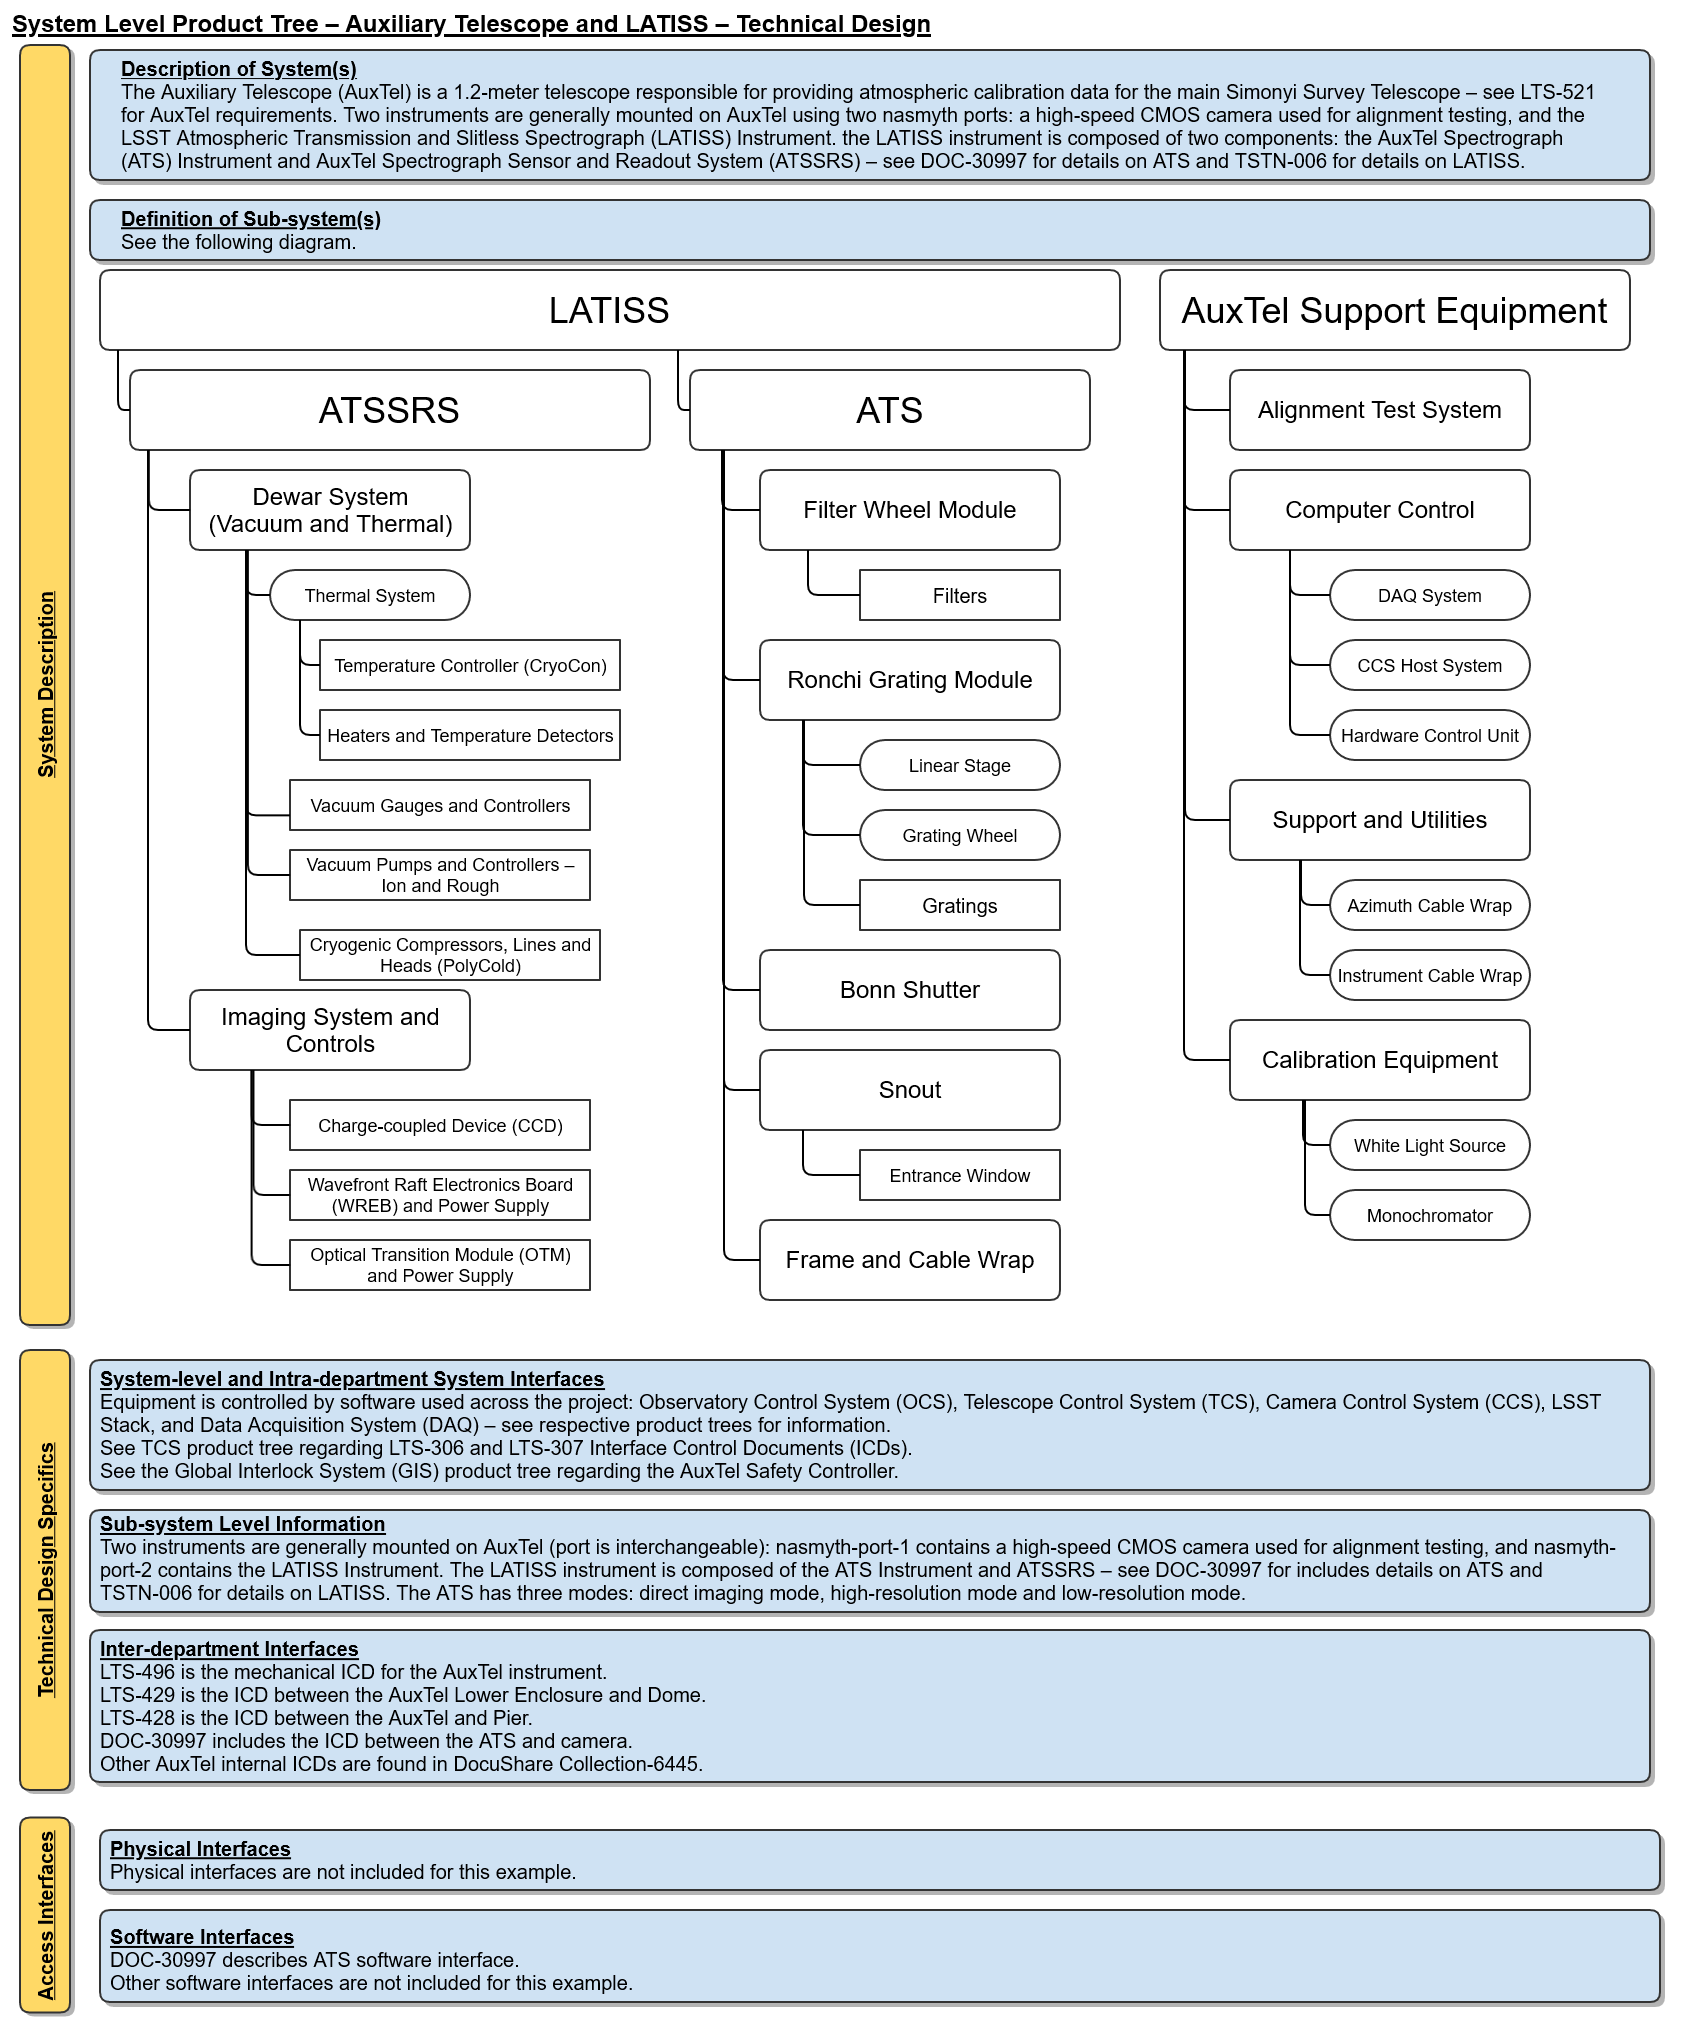
\includegraphics[width=\textwidth]{product-view-auxtel-product-tree-technical-design-example}
\caption{Example of Technical Design Generic Category from Product View, for an Auxiliary Telescope Subsystem.}
\label{fig:product-view-auxtel-technical-design-example}
\end{figure}

While it may seem Figure \ref{fig:product-view-departments-example} and Figure \ref{fig:product-view-auxtel-technical-design-example} are part of one example, that is not the case.
As previously described, it would be beneficial to organize the Product View to leverage the replicated information such as common software.
This was not considered for the two figures.

As another example of the Product View, Table \ref{table:product-view-department-ownership-example} shows how multiple departments can separate their responsibilities between a few high-level requirements and operational needs.
With well-defined responsibilities, teams can communicate more effectively and the normative source of information should be identifiable.

\begin{table}[]
\begin{tabular}{|l|l|l|l|}
\hline
 & \textbf{\begin{tabular}[c]{@{}l@{}}Rubin Observatory\\ Operations\end{tabular}} & \textbf{\begin{tabular}[c]{@{}l@{}}System\\ Performance\end{tabular}} & \textbf{\begin{tabular}[c]{@{}l@{}}Data\\ Management\end{tabular}} \\ \hline
\textbf{\begin{tabular}[c]{@{}l@{}}Technical\\ Design\end{tabular}} & \begin{tabular}[c]{@{}l@{}}ICDs/IDDs\\ Requirements\end{tabular} & \begin{tabular}[c]{@{}l@{}}Validation of\\ Science Platform\end{tabular} & \begin{tabular}[c]{@{}l@{}}Science Platform\\ Design and Operations\end{tabular} \\ \hline
\textbf{Procedures} & \begin{tabular}[c]{@{}l@{}}Day/Night Shift Turn-over,\\ Energy Isolation Protocols,\\ Calibration Procedures\end{tabular} & \begin{tabular}[c]{@{}l@{}}Predictive Analysis,\\ Hazard Validation\end{tabular} & \begin{tabular}[c]{@{}l@{}}Data Release and\\ Prompt Alerts\\ Processing\end{tabular} \\ \hline
\textbf{Evaluation} & \begin{tabular}[c]{@{}l@{}}Verification Test Plans,\\ Failure Effects,\\ Test Reports\end{tabular} & \begin{tabular}[c]{@{}l@{}}Failure Mode and\\ Effect Analysis\end{tabular} & \begin{tabular}[c]{@{}l@{}}Assertion\\ Testing\end{tabular} \\ \hline
\end{tabular}
\label{table:product-view-department-ownership-example}
\end{table}
